\newpage
\mysection{Appendix}

\mysubsection{GoogLeNet - InceptionV1 architecture}
\begin{figure}[htbp]
\centering
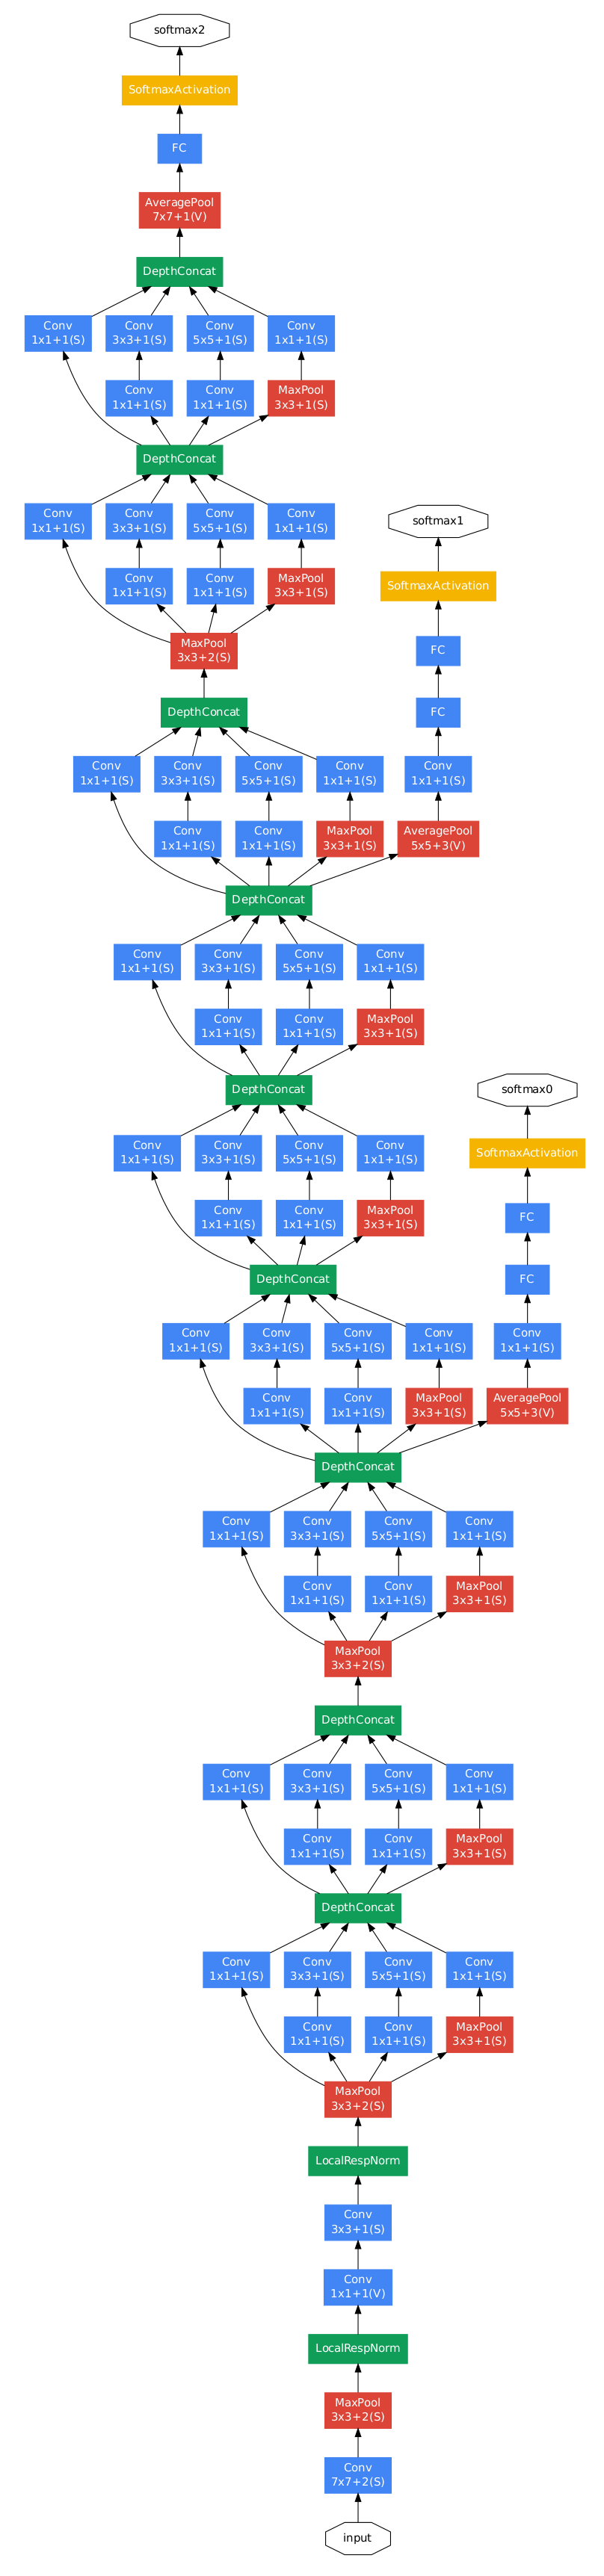
\includegraphics[height=18.5cm]{includes/GoogLeNet}
\caption[Model architecture of GoogLeNet]{Model architecture of GoogLeNet \citep[p. 7]{Szegedy2014}}
\label{fig:GoogLeNet}
\end{figure}
\newpage


\mysubsection{ResNet architecture}
\begin{figure}[htbp]
\centering
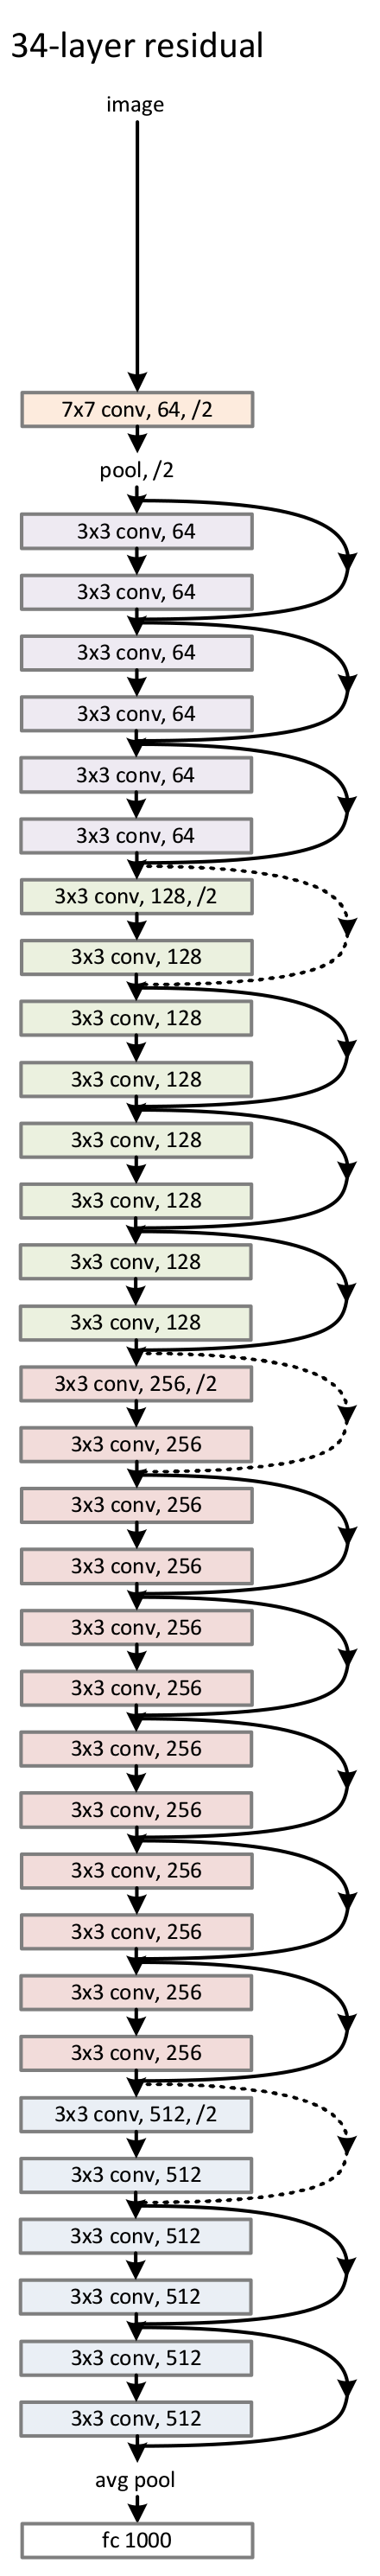
\includegraphics[height=18.5cm]{includes/ResNet}
\caption[ResNet block]{ResNet block \citep[p. 4]{HE2015}}
\label{fig:FH-Logo6}
\end{figure}
\newpage


\mysubsection{Configure Bazel for Tensorflow}

\begin{lstlisting}[caption=Configure bazel for Tensorflow, label=list:configure_bazel, language=bash]
	$ cd tensorflow  # cd to the top-level directory created
	$ ./configure
	Please specify the location of python. [Default is /usr/bin/python]: /usr/bin/python3.6
	Found possible Python library paths:
	  /usr/local/lib/python3.6/dist-packages
	  /usr/lib/python3.6/dist-packages
	Please input the desired Python library path to use.  Default is [/usr/lib/python3.6/dist-packages]
	Using python library path: /usr/local/lib/python3.6/dist-packages
	Do you wish to build TensorFlow with MKL support? [y/N]
	No MKL support will be enabled for TensorFlow
	Please specify optimization flags to use during compilation when bazel option "--config=opt" is specified [Default is -march=native]:
	Do you wish to use jemalloc as the malloc implementation? [Y/n] n
	No jemalloc as malloc support will be enabled for TensorFlow.
	Do you wish to build TensorFlow with Google Cloud Platform support? [y/N] n
	No Google Cloud Platform support will be enabled for TensorFlow
	Do you wish to build TensorFlow with Hadoop File System support? [y/N] n
	No Hadoop File System support will be enabled for TensorFlow
	Do you wish to build TensorFlow with the XLA just-in-time compiler (experimental)? [y/N] n
	No XLA support will be enabled for TensorFlow
	Do you wish to build TensorFlow with Amazon S3 File System support? [Y/n]: n
	No Amazon S3 File System support will be enabled for TensorFlow.
	Do you wish to build TensorFlow with GDR support? [y/N]: n
	No GDR support will be enabled for TensorFlow.
	Do you wish to build TensorFlow with VERBS support? [y/N] n
	No VERBS support will be enabled for TensorFlow
	Do you wish to build TensorFlow with OpenCL support? [y/N] n
	No OpenCL support will be enabled for TensorFlow
	Do you wish to build TensorFlow with CUDA support? [y/N] Y
	CUDA support will be enabled for TensorFlow
	Please specify the Cuda SDK version you want to use, e.g. 7.0. [Leave empty to default to CUDA 8.0]: 8.0
	Please specify the location where CUDA 8.0 toolkit is installed. Refer to README.md for more details. [Default is /usr/local/cuda]:
	Please specify the cuDNN version you want to use. [Leave empty to default to cuDNN 6.0]: 6
	Please specify the location where cuDNN 6 library is installed. Refer to README.md for more details. [Default is /usr/local/cuda]:
	Please specify a list of comma-separated Cuda compute capabilities you want to build with.
	You can find the compute capability of your device at: https://developer.nvidia.com/cuda-gpus.
	Please note that each additional compute capability significantly increases your build time and binary size.
	[Default is: 5.2]: 5.2
	Do you want to use clang as CUDA compiler? [y/N] n
	nvcc will be used as CUDA compiler
	Please specify which gcc should be used by nvcc as the host compiler. [Default is /usr/bin/gcc]:
	Do you wish to build TensorFlow with MPI support? [y/N] n
	MPI support will not be enabled for TensorFlow
	Configuration finished
\end{lstlisting}

\begin{sidewaysfigure}
\mysubsection{Mobile Application Architecture in the form of a Class Diagram}
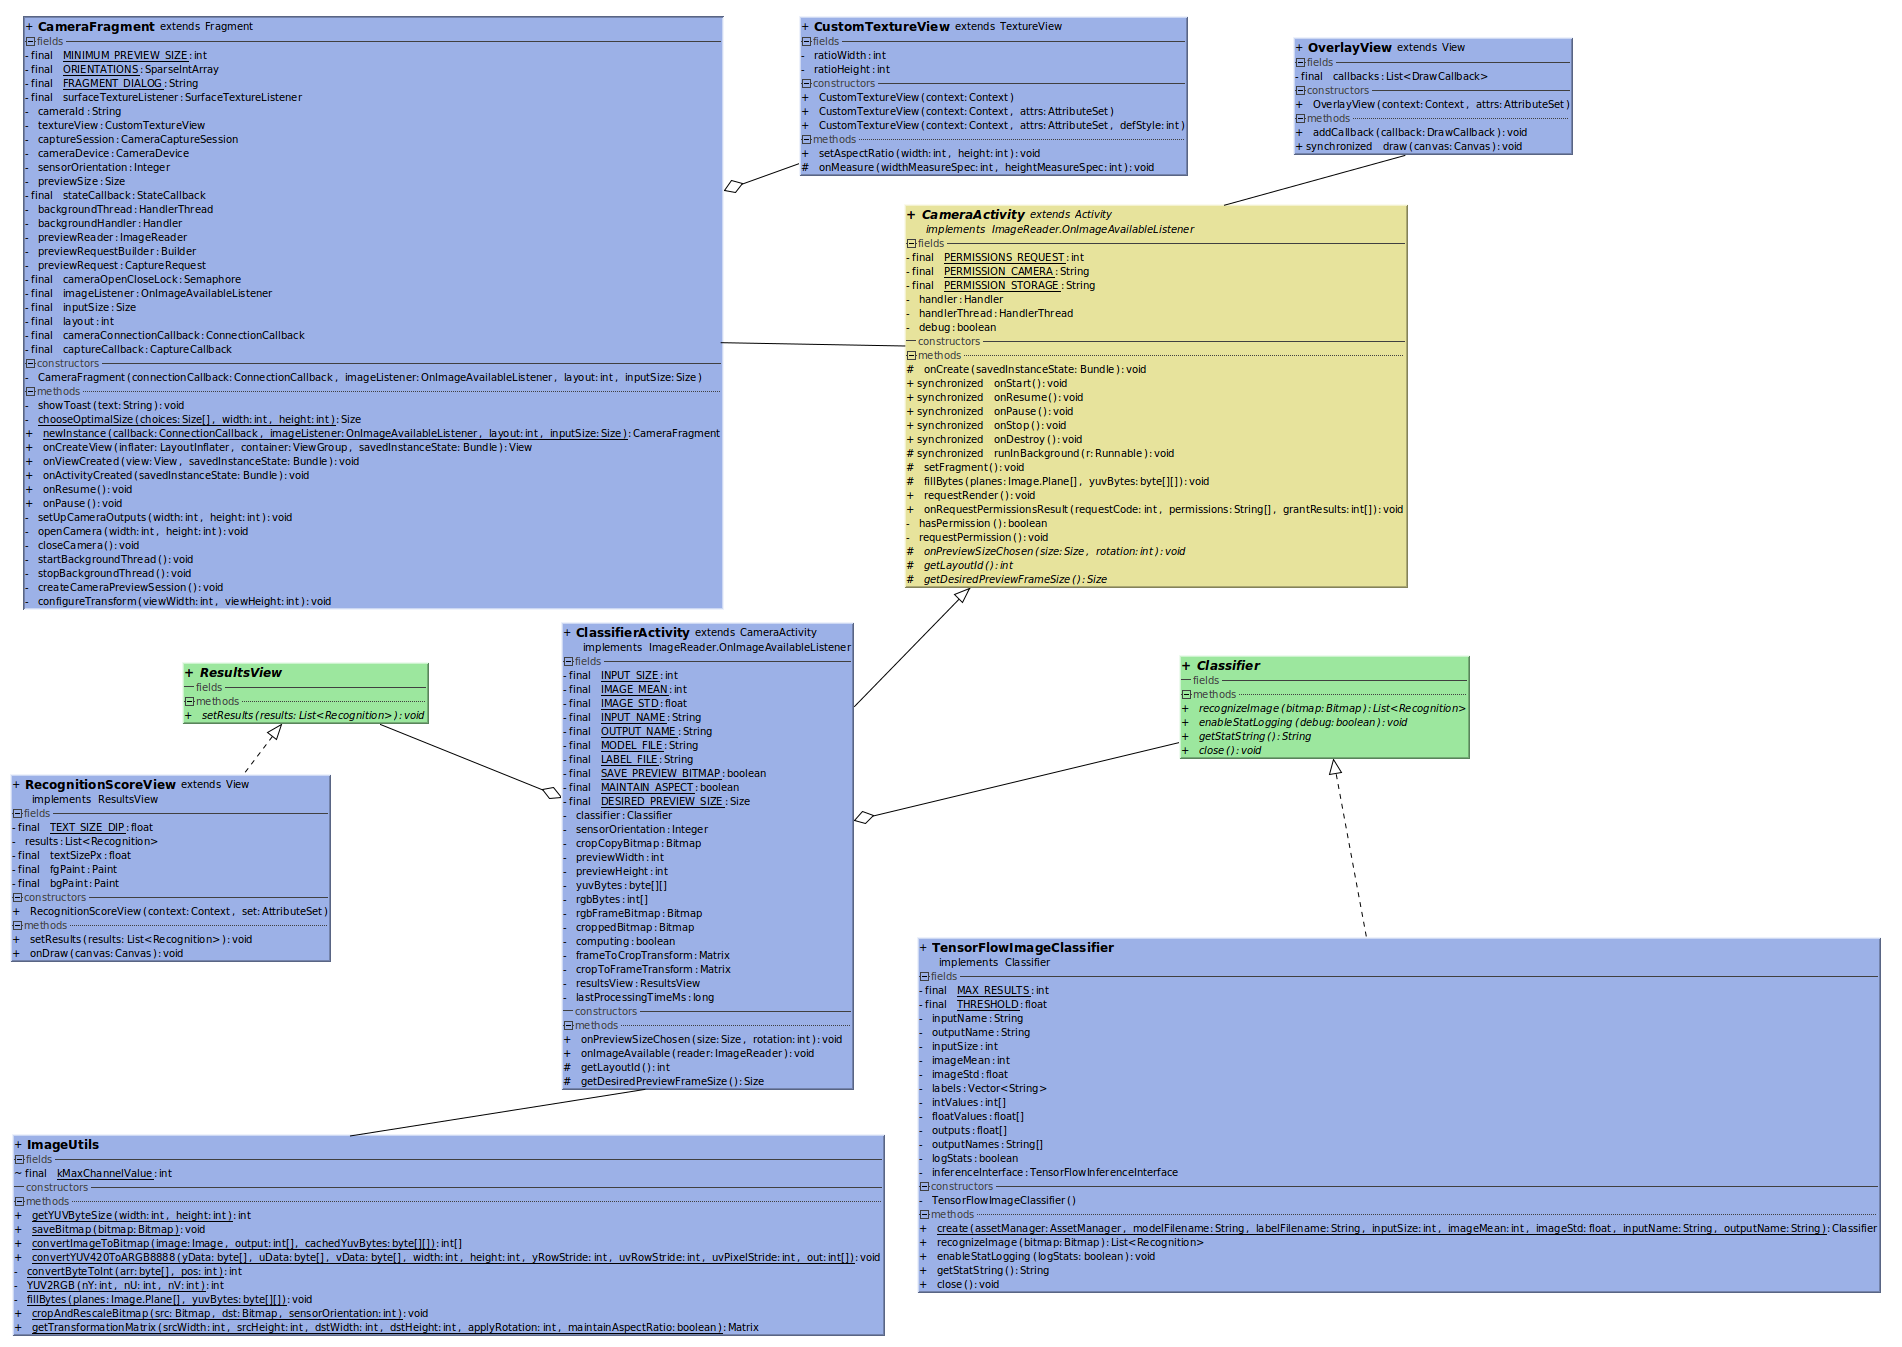
\includegraphics[width=0.95\textwidth]{includes/ClassDiagram}
\end{sidewaysfigure}
\newpage


\mysubsection{MobileNet retrained graph - detailed}
\begin{figure}[htbp]
\centering
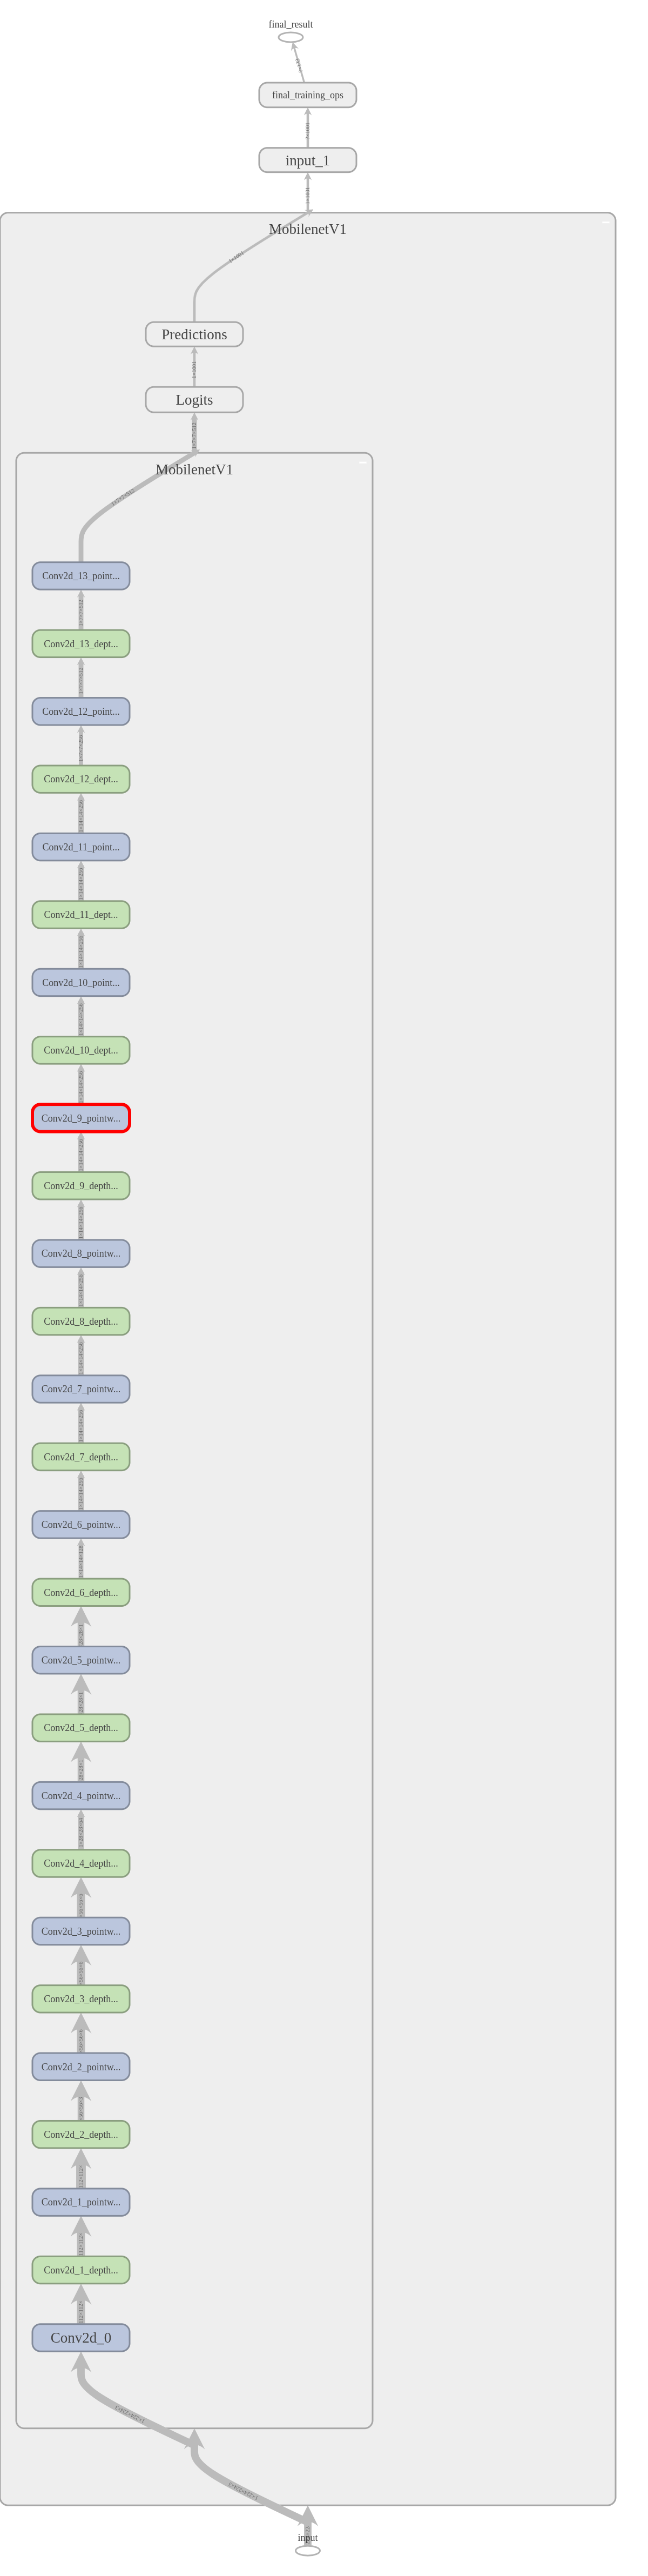
\includegraphics[height=18.5cm]{includes/graphMobilenet050-700Layer}
\caption{MobileNet retrained graph - detailed}
\label{fig:MobileNet retrained graph - detailed}
\end{figure}
\newpage

\mysubsection{MobileNet retrained graph - depthwise}
\begin{figure}[htbp]
\centering
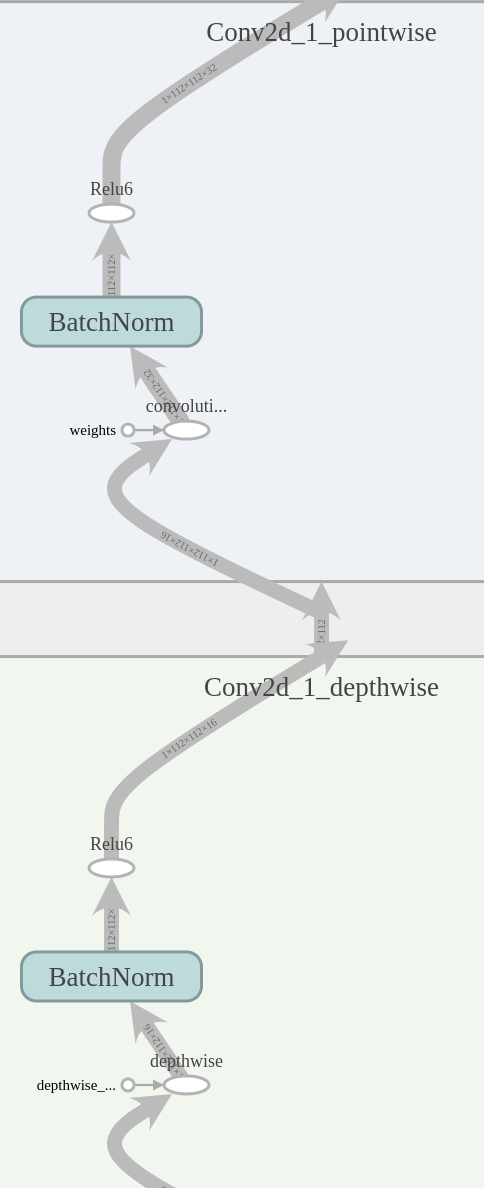
\includegraphics[height=10cm]{includes/graphMobilenet050-700DepthLayer}
\caption{MobileNet retrained graph - depthwise}
\label{fig:MobileNet retrained graph - depthwise}
\end{figure}

\newpage


\mysubsection{InceptionV3 retrained graph}
\begin{figure}[htbp]
\centering
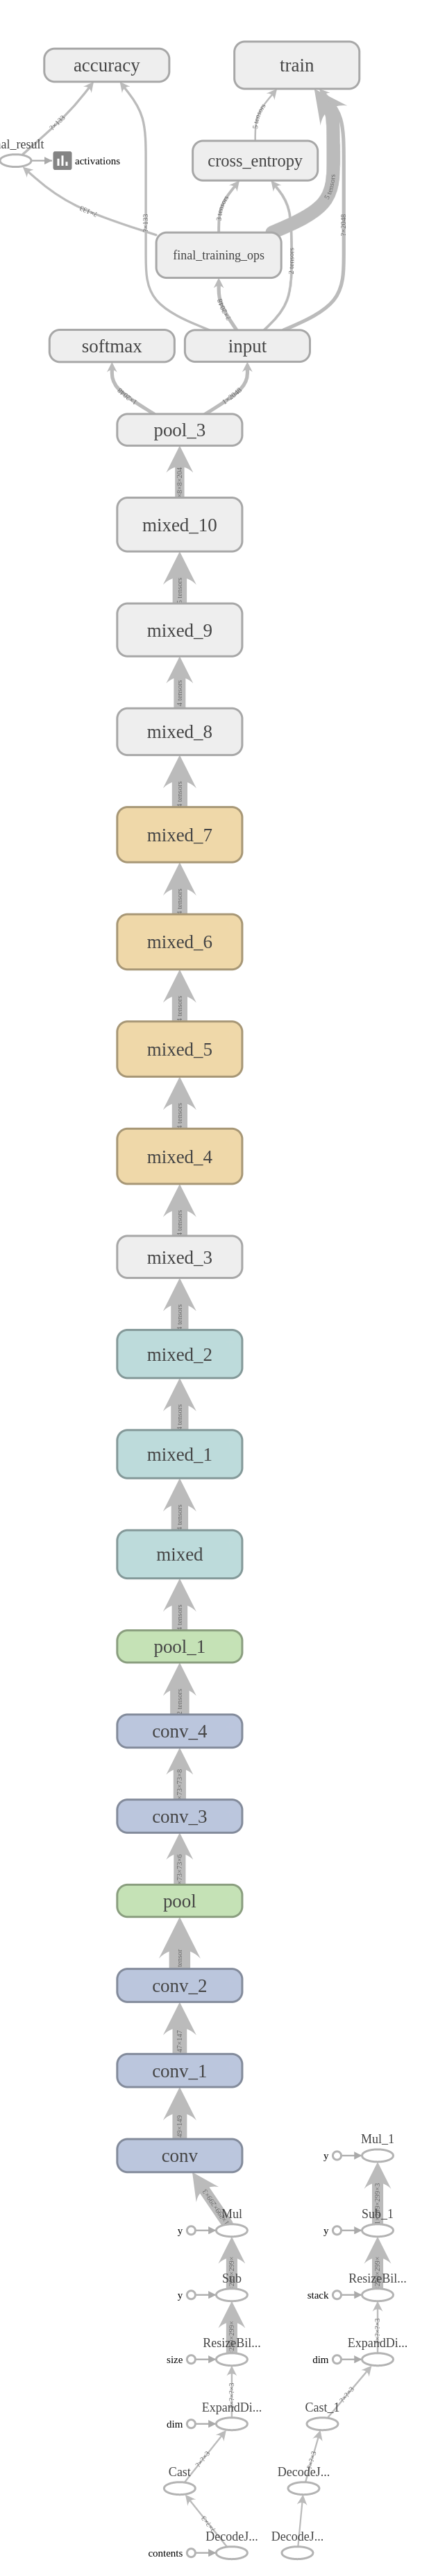
\includegraphics[height=18.5cm]{includes/graphInception4000}
\caption{InceptionV3 retrained graph}
\label{fig:InceptionV3 retrained graph}
\end{figure}

\begin{sidewaysfigure}
\mysubsection{InceptionV3 retrained graph - mixed_layer}
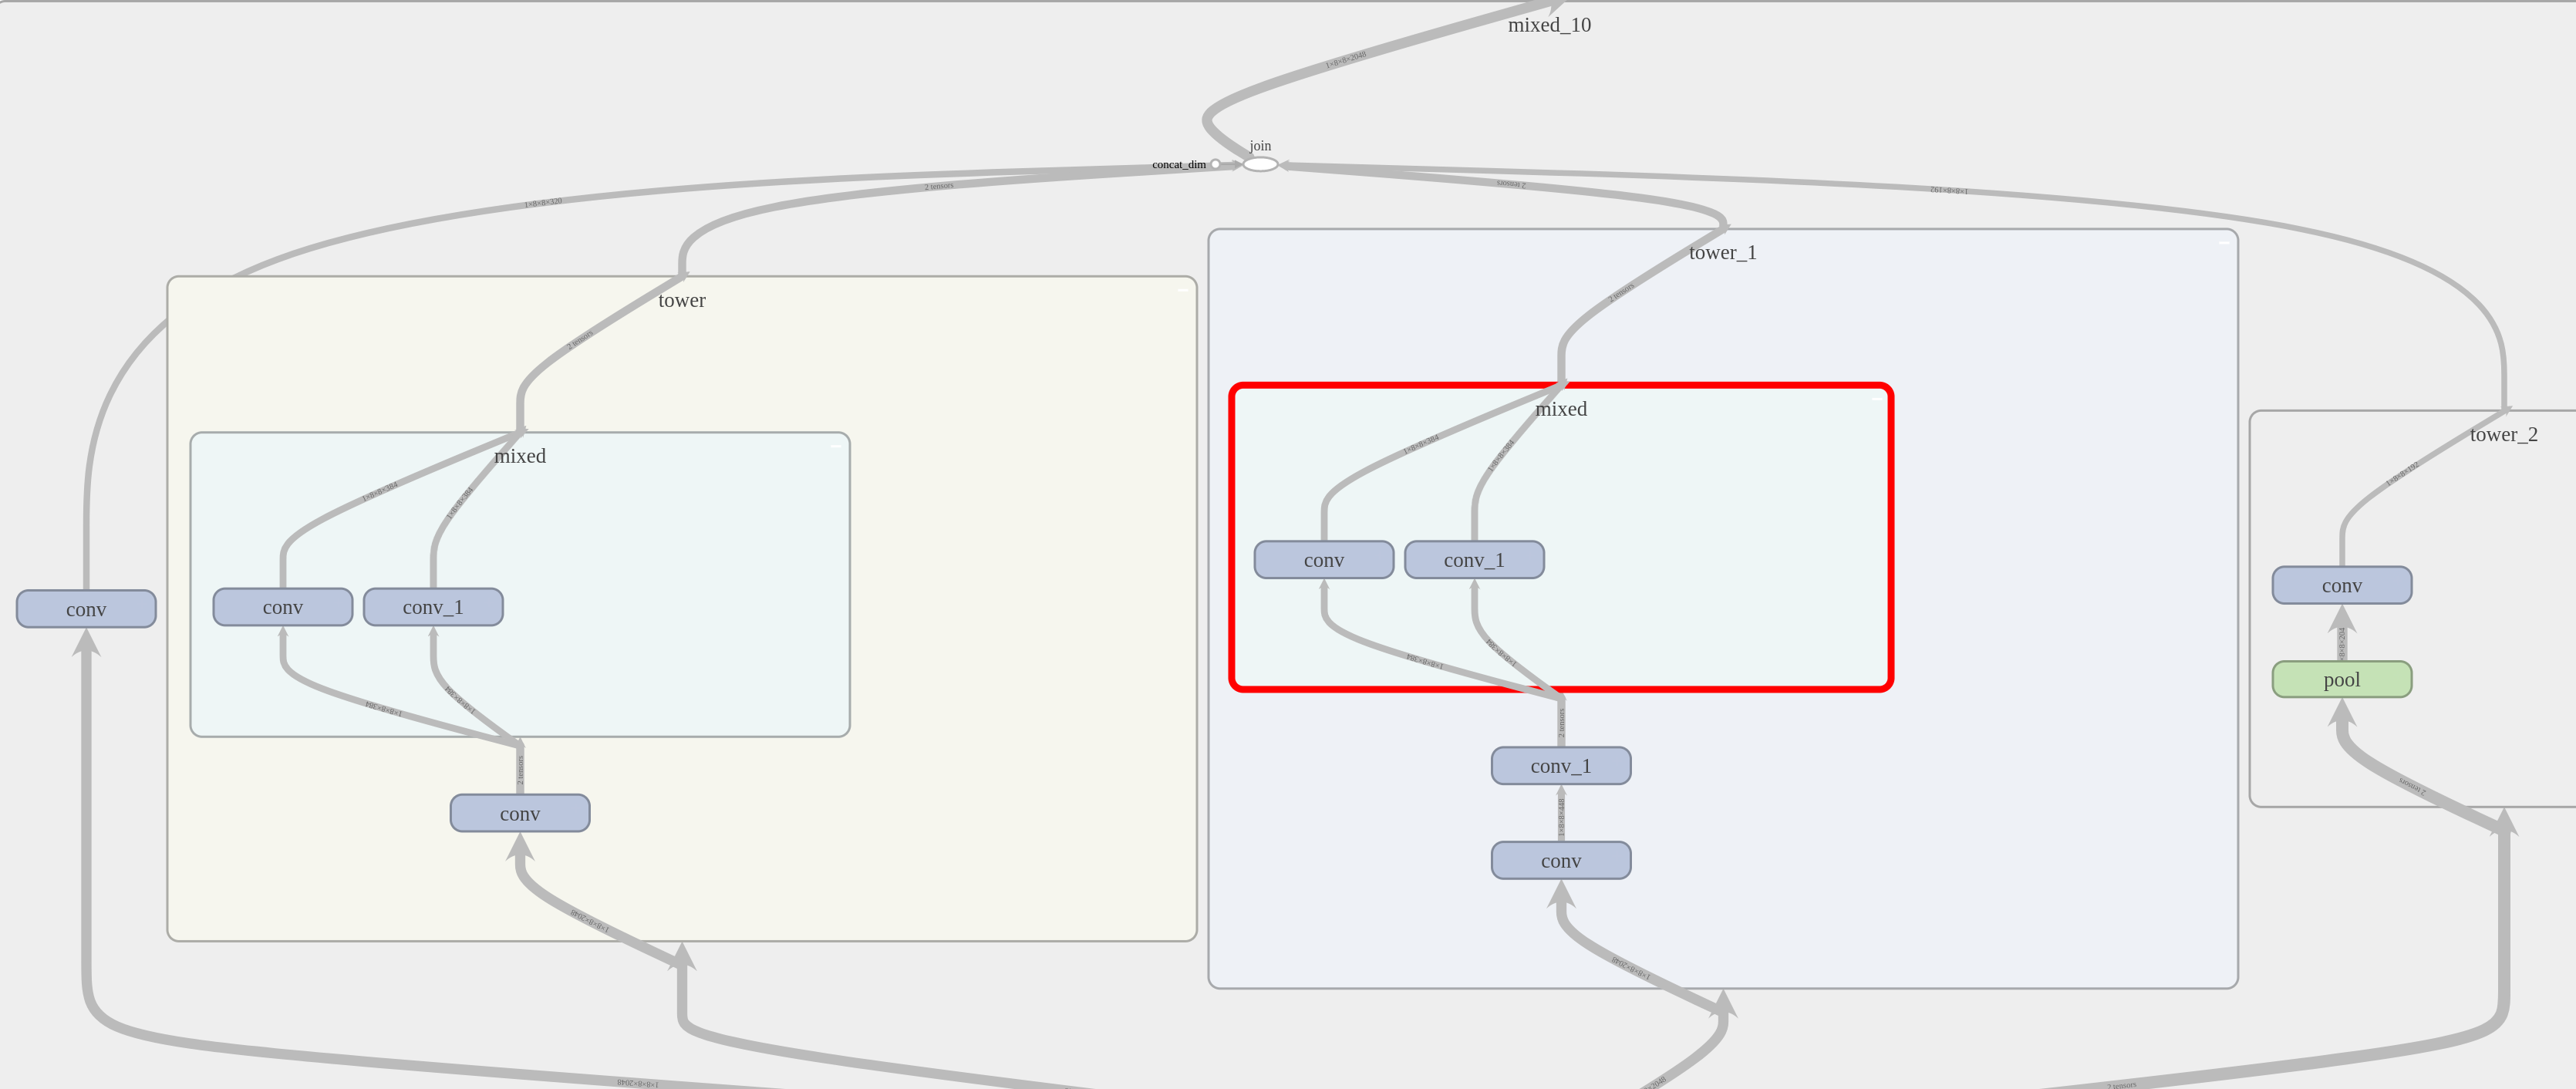
\includegraphics[width=0.95\textwidth]{includes/graphInception4000MixedLayer}
\end{sidewaysfigure}
\newpage

\mysubsection{InceptionV3 retrained graph - conv layer}
\begin{figure}[htbp]
\centering
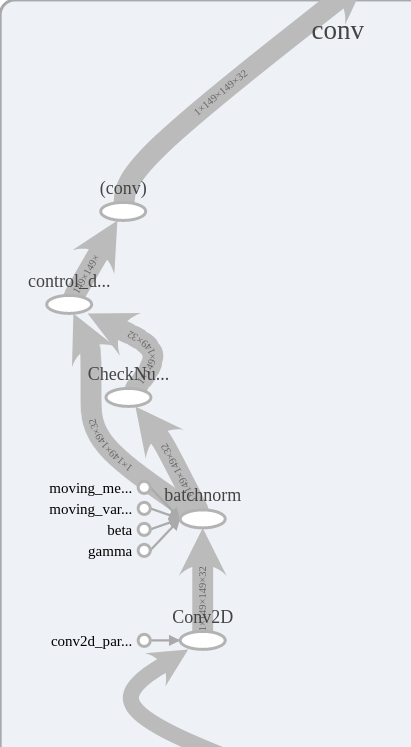
\includegraphics[width=0.35\textwidth]{includes/graphInception4000ConvOps1}
\caption{InceptionV3 retrained graph - conv layer}
\label{fig:InceptionV3 retrained graph - conv layer}
\end{figure}
\newpage

\mysubsection{InceptionV3 retrained graph - optimized}
\begin{figure}[htbp]
\centering
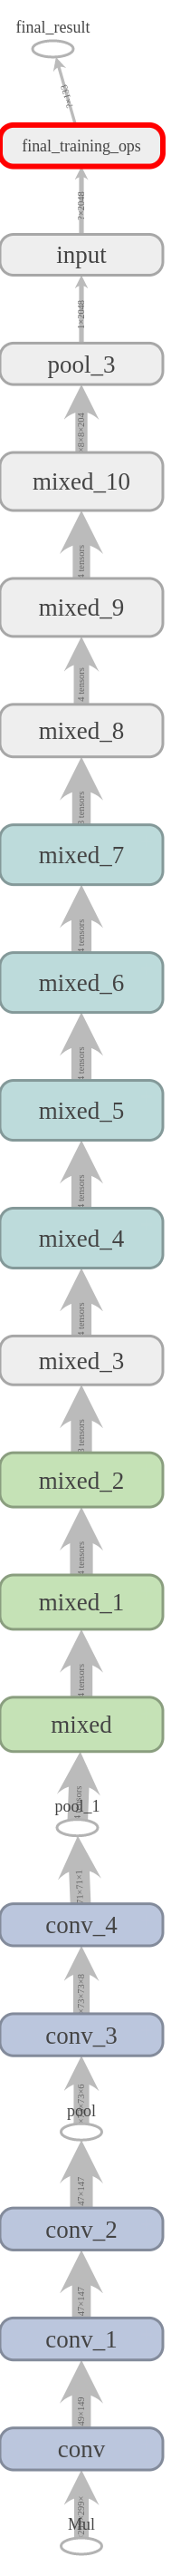
\includegraphics[height=18.5cm]{includes/graphInception4000Opt4}
\caption{InceptionV3 retrained graph - optimized}
\label{fig:InceptionV3 retrained graph - optimized}
\end{figure}
\newpage

\mysubsection{TensorBoard - optimal achieved accuracy of the different models}
\begin{figure}[htbp]
\centering
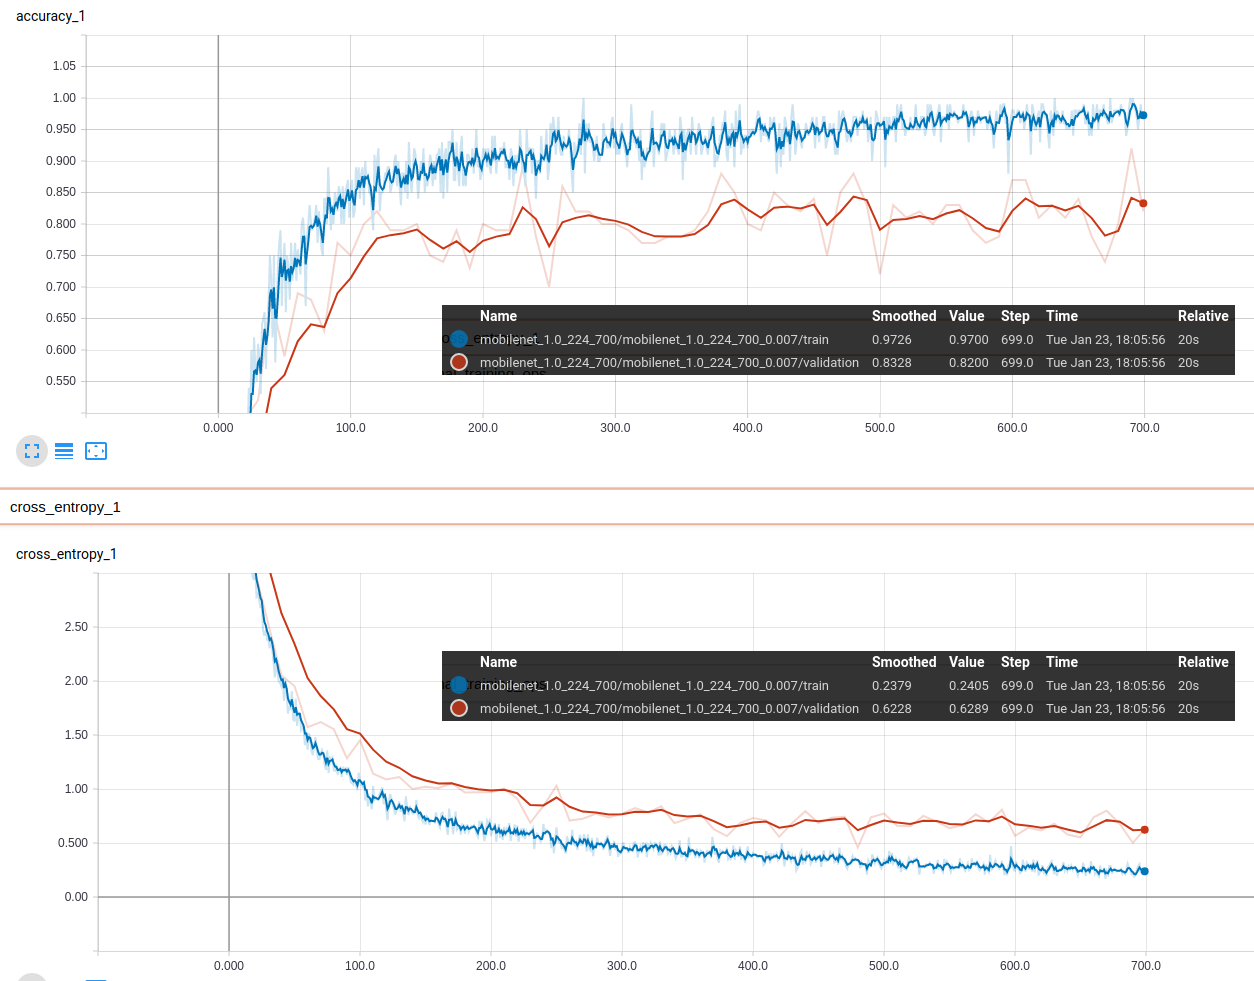
\includegraphics[width=0.95\textwidth]{includes/MobileNet05-700res}
\caption{TensorBoard - optimal achieved accuracy of MobileNet_0.5}
\label{fig:MobileNet05-700res}
\end{figure}

\begin{figure}[htbp]
\centering
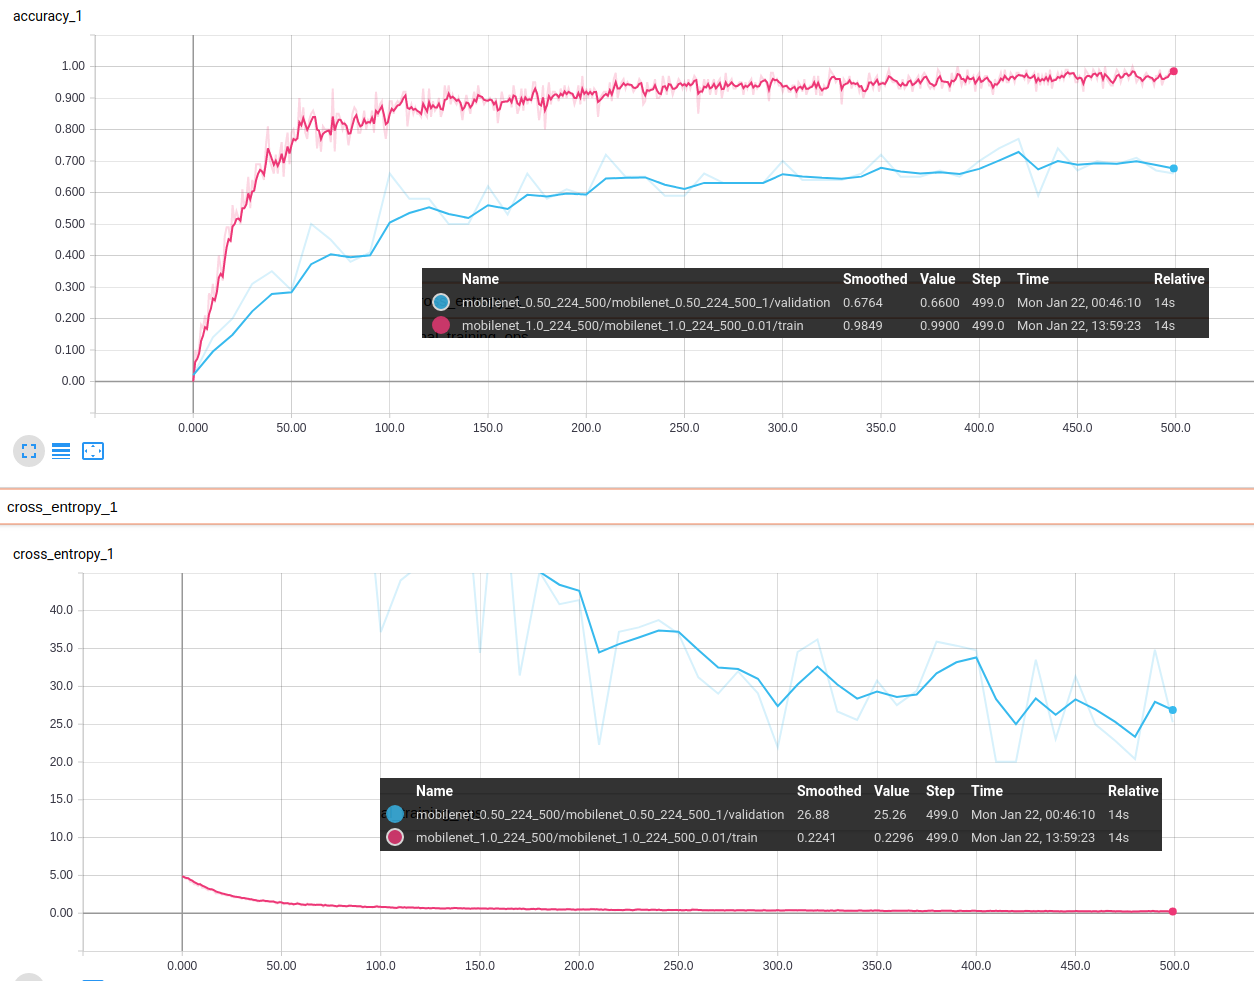
\includegraphics[width=0.95\textwidth]{includes/MobileNet10-500res}
\caption{TensorBoard - optimal achieved accuracy of MobileNet_1.0}
\label{fig:MobileNet10-500res}
\end{figure}

\begin{figure}[htbp]
\centering
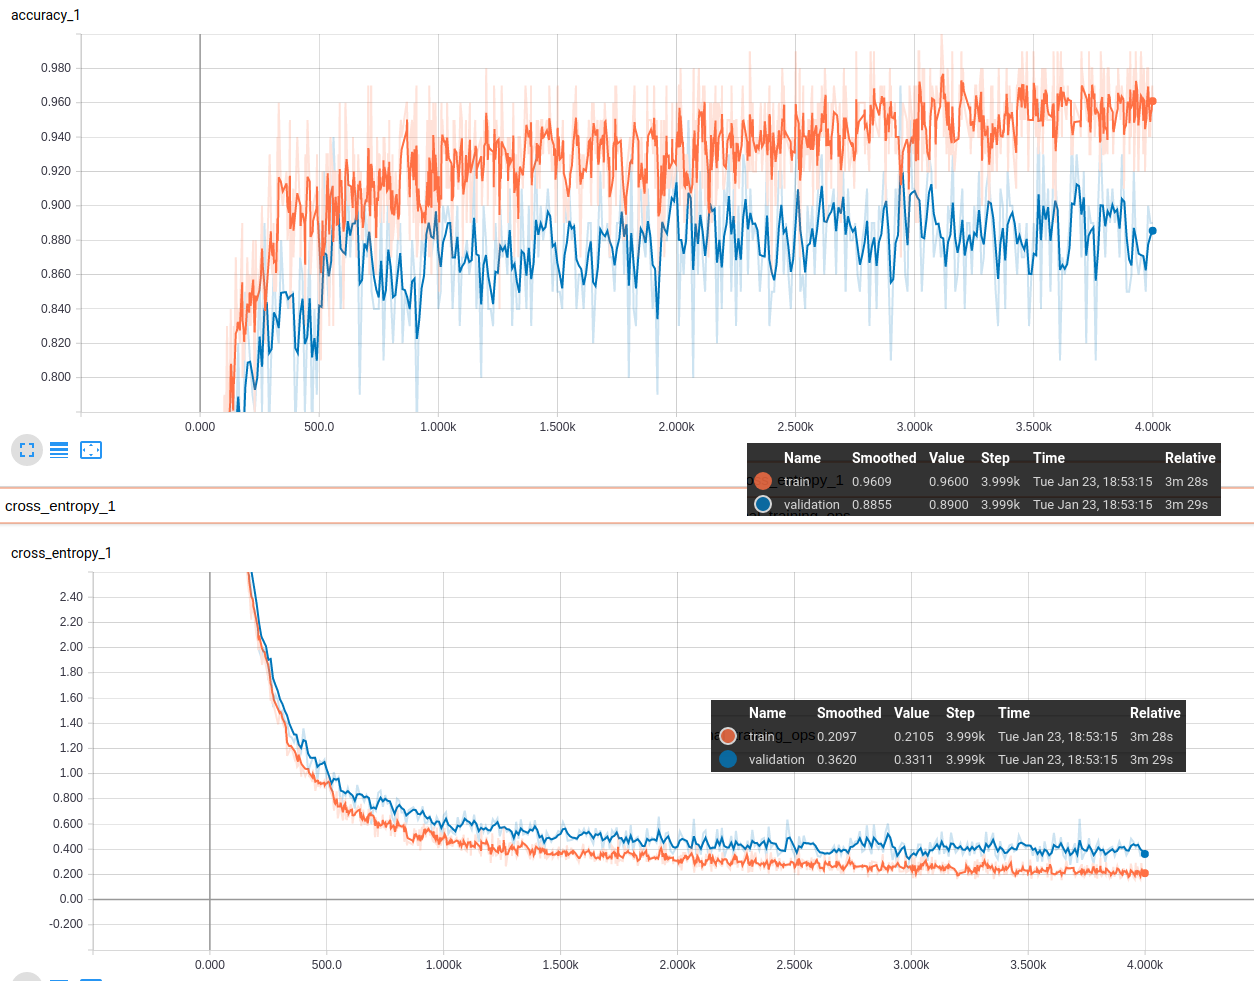
\includegraphics[width=0.95\textwidth]{includes/inception4000res}
\caption{TensorBoard - optimal achieved accuracy of InceptionV3}
\label{fig:inception4000res}
\end{figure}

\begin{figure}[htbp]
\centering
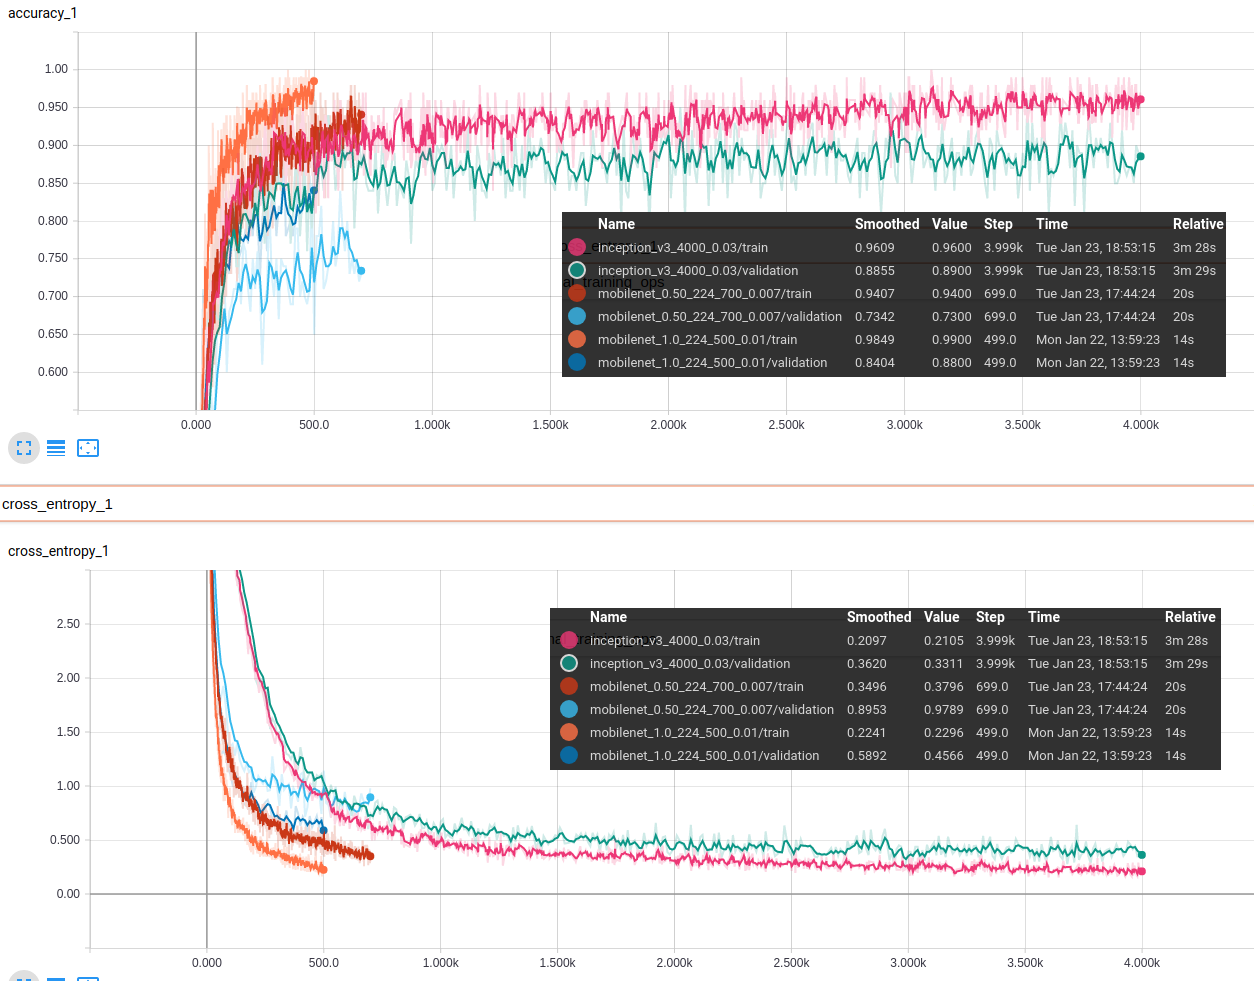
\includegraphics[width=0.95\textwidth]{includes/AllRes}
\caption{TensorBoard - optimal achieved accuracy of all models}
\label{fig:AllRes}
\end{figure}

\newpage

\mysubsection{Evaluation of optimization attempts}

\newpage
\begin{table}[]
\centering
\begin{tabular}{|l|r|r|r|l}
\cline{1-4}
opt attempt & \multicolumn{1}{l|}{accuracy} & \multicolumn{1}{l|}{misclassified} & \multicolumn{1}{l|}{time to classify (App) {[}ms{]}} &  \\ \cline{1-4}
retrained & 0,566641033                   & 5                                           & 0                                &  \\ \cline{1-4}
opt1      & 0,566641033                   & 5                                           & 239,6                           &  \\ \cline{1-4}
opt2      & 0,487681977                   & 8                                           & 252,5                           &  \\ \cline{1-4}
opt3      & 0,566641033                   & 5                                           & 241,9                   &  \\ \cline{1-4}
opt4      & 0,483819713                   & 8                                           & 246,8                            &  \\ \cline{1-4}
\end{tabular}
\caption{MobileNet_0.5}
\label{tab:mobileNet05}
\end{table}

\begin{table}[]
\centering
\begin{tabular}{|l|r|r|r|l}
\cline{1-4}
opt attempt & \multicolumn{1}{l|}{accuracy} & \multicolumn{1}{l|}{misclassified} & \multicolumn{1}{l|}{time to classify (App) {[}ms{]}} &  \\ \cline{1-4}
retrained & 0,504834563                   & 7                                           & 0                                &  \\ \cline{1-4}
opt1      & 0,504834563                   & 7                                           & 316,2                            &  \\ \cline{1-4}
opt2      & 0,458024049                   & 8                                           & 310,2                           &  \\ \cline{1-4}
opt3      & 0,504834563                   & 7                                           & 323,4                            &  \\ \cline{1-4}
opt4      & 0,458474453                   & 8                                           & 320,6                           &  \\ \cline{1-4}
\end{tabular}
\caption{MobileNet_1.0}
\label{tab:mobileNet10}
\end{table}

\begin{table}[]
\centering
\begin{tabular}{|l|r|r|r|l}
\cline{1-4}
opt attempt & \multicolumn{1}{l|}{accuracy} & \multicolumn{1}{l|}{misclassified} & \multicolumn{1}{l|}{time to classify (App) {[}ms{]}} &  \\ \cline{1-4}
retrained   & 0,722748141                   & 2                                           & 0                                                    &  \\ \cline{1-4}
opt1        & 0,722748250                   & 2                                           & 1092,2                                              &  \\ \cline{1-4}
opt2        & 0,698508064                   & 3                                           & 1094,4                                               &  \\ \cline{1-4}
opt3        & 0,722748137                   & 2                                           & 1139,9                                               &  \\ \cline{1-4}
opt4        & 0,700055786                   & 3                                           & 1108,2                                               &  \\ \cline{1-4}
\end{tabular}
\caption{InceptionV3}
\label{tab:inception}
\end{table}
